\section{Sistēmas pārskats}
Sistēmai tiek izvēlēti 2 industriālā tipa AC-DC barošanas avoti "CUS800M-24" \cite{24v_industrial_ps} un "LRS-150-12" \cite{12v_industrial_ps}, kas nodrošina no 230VAC uz 24 VDC un 12 VDC barošanu sistēmai. 24 V barošanas avots HPA jaudas nodrošināšanai. Pirms spriegums tiek padots HPA notecēm, barošāna iet cauri ieslēgšanas/izslēgšanas slēdzim, kas tiek vadīts ar AD7293 integrālo shēmu. Tālāk tiek mērīta plūstošā strāva ar šunta rezistoriem, līdz tā nonāk pie HPA bloka diviem jaudas pastiprinātājiem. Jaudas pastiprinātāja signāla traktā no frekvenču augšupārveidotāja ienāk signāls, kas tiek pastiprināts +50 dBm. Pastiprinātais signāls iet cauri atzarotājam, kas paredzēts izstarotās un atstarotās jaudas mērīšanai, kur 0 dBm atbilst 100 W un -50 dBm atbilst 1 mW uz $P_{fwd}$ un $P_{refl}$. Pēc atzarotāja pastiprinātais ieejas signāls nonāk RT-16 antenā un tālāk tiek raidīts dziļajā kosmosā. 12 V barošanas avots nodrošina jaudu ciparu elektronikai un jaudas mērītājam. 12 V tiek pārveidoti uz 9 un 5 V. 9 V tiek nodrošināti monitorēšanas integrālajai shēmai, bet 5 V mikrokontrolierim, temperatūras sensoram un vidējās jaudas mērītājam. RMS detektors mēra izstaroto un atstaroto jaudu, kur izejas sprieguma līmenis atbilst noteiktai jaudai dBm, kur tas tiek padots uz monitorēšanas sistēmu. Mikrokontrolieris konfigurē monitorēšanas sistēmu un mēra HPA temperatūru. Pie monitorēšanas sistēmas arī ir 2 ārējie temperatūras sensori, kas arī mēra HPA temperatūru. No kontroles/operatora datora tiek nosūtītas komandas uz mikrokontrolieri caur TCP protokolu lokālā tīklā.
\begin{figure}[H]
	\centering
    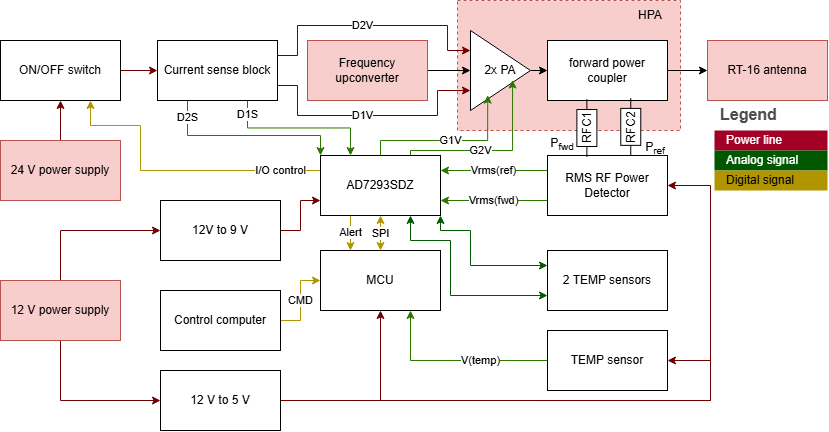
\includegraphics[width=0.9\textwidth]{pictures/project_diagram.png}\hspace{1cm}
    \caption{Vadības bloka augsta līmeņa bloka diagramma}
\end{figure}

